\subsection{UC6 - Selezione distanza}
\label{uc6}

    \begin{figure}[htbp]
        \centering
        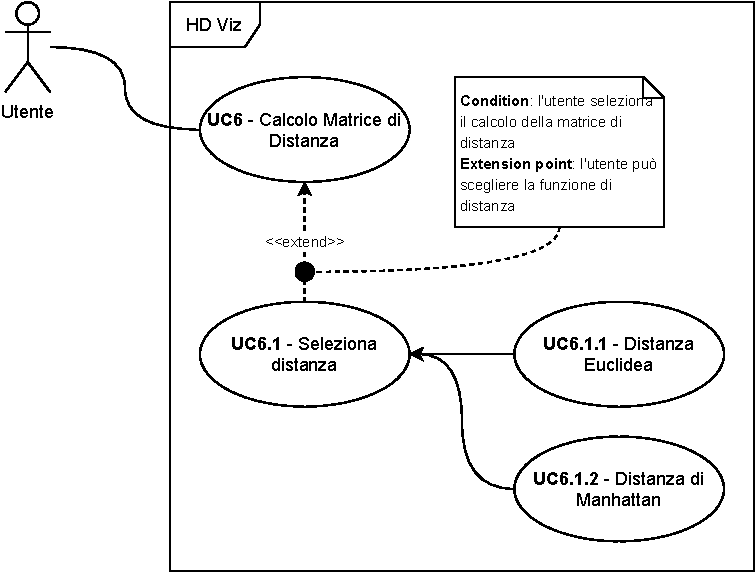
\includegraphics[width=0.45\textwidth]{source/sections/casi-uso/diagrams/uc6.pdf}
        \caption{UC6 - Selezione distanza}
        \label{fig:uc6}
    \end{figure}
    
    \begin{itemize}
    \item \textbf{Attore}: utente;
    \item \textbf{Descrizione}: l'utente sceglie la distanza da utilizzare durante l'elaborazione dati;
    \item \textbf{Precondizione}: 
    \begin{itemize}
        \item eseguito l'upload del dataset come matrice $N\times M$ (\hyperref[uc1]{UC1}).
        \item selezionato Heatmap o Force Field come visualizzazione (\hyperref[uc2.2]{UC2.2} o \hyperref[uc2.4]{UC2.4}).
        \item selezionato calcola matrice di distanza (\hyperref[uc5]{UC5}).
    \end{itemize}  
    \item \textbf{Postcondizione}: l'utente ha scelto la distanza da utilizzare;
    \item \textbf{Scenario Principale}: 
    \begin{enumerate}
        \item l'utente seleziona la distanza tra quelle disponibili.
    \end{enumerate}
    \item \textbf{Generalizzazioni}:
        \begin{enumerate}
            \item l'utente seleziona una delle seguenti distanze:
                \begin{enumerate}
                    \item Euclidea (\hyperref[uc6.1]{UC6.1});
                    \item Manhattan (\hyperref[uc6.2]{UC6.2}).
                \end{enumerate}
        \end{enumerate}  
    \end{itemize}
    
    \paragraph{UC6.1 - Distanza euclidea}
    \label{uc6.1}
    \begin{itemize}
    \item \textbf{Attore}: utente;
    \item \textbf{Descrizione}: l'utente sceglie la distanza \emph{Euclidea};
    \item \textbf{Precondizione}: 
    \begin{itemize}
        \item eseguito l'upload del dataset come matrice $N\times M$ (\hyperref[uc1]{UC1});
        \item selezionato Heatmap o Force Field come visualizzazione (\hyperref[uc2.2]{UC2.2} o \hyperref[uc2.4]{UC2.4}).
        \item selezionato calcola matrice di distanza (\hyperref[uc5]{UC5}).
    \end{itemize}  
    \item \textbf{Postcondizione}: l'utente ha scelto la distanza euclidea;
    \item \textbf{Scenario Principale}: 
    \begin{enumerate}
        \item l'utente ha scelto la distanza euclidea.
    \end{enumerate}
    \end{itemize}
    
    \paragraph{UC6.2 - Distanza di Manhattan}
    \label{uc6.2}
    \begin{itemize}
    \item \textbf{Attore}: utente;
    \item \textbf{Descrizione}: l'utente sceglie la distanza di \emph{Manhattan};
    \item \textbf{Precondizione}: 
    \begin{itemize}
        \item eseguito l'upload del dataset come matrice $N\times M$ (\hyperref[uc1]{UC1});
        \item selezionato Heatmap o Force Field come visualizzazione (\hyperref[uc2.2]{UC2.2} o \hyperref[uc2.4]{UC2.4}).
        \item selezionato calcola matrice di distanza (\hyperref[uc5]{UC5}).
    \end{itemize}  
    \item \textbf{Postcondizione}: l'utente ha scelto la distanza di Manhattan;
    \item \textbf{Scenario Principale}: 
    \begin{enumerate}
        \item l'utente ha scelto la distanza di Manhattan.
    \end{enumerate}
    \end{itemize}
